\documentclass{article}
\usepackage[utf8]{inputenc}
\usepackage{cite}
\usepackage{geometry}
\usepackage{amsmath}
\usepackage{pythontex}
\usepackage{graphicx}
\usepackage{float}

\title{Integrating Continuous Credentials in Authentication
Mechanisms}
\author{Dor Malka, Ittay Eyal}
\date{\today}

\begin{document}

\maketitle

\section{Abstract}
%%%
%%%
%%%
Authentication is a fundamental aspect of security that can be viewed from two main perspectives: credentials and protocols. The credentials aspect is familiar to most of us through username and password, or OTPs used when accessing personal bank account or authenticating into services such as Google/Apple ID. While these discrete credentials, which rely on simply having or knowing something are widely used, there remains a largely unexplored space: continuous credentials.

Continuous credentials appear in several applications such as biometric authentication (fingerprints, eigenface or iris) and SSO mechanisms that rely on behavioral or environmental signals like GPS location etc. These credentials are not evaluated in a discrete way. Rather, they are measured by a mechanism that determines whether there are enough similarities above a predetermined threshold between an input and a stored figure.

These mechanisms introduce a spectrum of confidence instead of a strict yes or no decision. As achieving high security level based on one credential and satisfying the mechanism might be hard, we aim to study the integration of several continuous credentials. Our research will explore how multiple continuous credentials can be fused to form a robust authentication mechanism and determine an optimal mechanism, achieving high security level in wallet design for both digital and physical assets.
\section{Related Work}
Lin Hong et al.~\cite{hong1998} found that automatic personal identification system based solely on fingerprints or faces is often not able to reach sufficiently low FAR and FRR. They integrated a biometric system which makes personal identification by integrating both faces and fingerprints operates during identification mode. The decision fusion of their system is designed to operate at measurement level, that is the system doesn’t just output a single decision or label but rather a set of labels with confidence values. The system decision is based on the confidence of each one of the modules which might lead to a more reliable and informative overall confidence score.

These confidence values are characterized by the FAR values of the credential. The FAR values were calculated as the number of similarities between 2 measures above a threshold t. If there are 5 similarities out of 8 between 2 fingerprints and the threshold was 4, these 2 fingerprints will be considered equal.

Prabhakar et al.~\cite{prabhakar2003} examined the tradeoff between False Acceptance Rate (FAR) and False Rejection Rate (FRR), highlighting its impact on both the accuracy and security of biometric systems. Their findings suggest that most applications aim to operate at a point that balances these two metrics.

This concept is further developed by Sarkar et al.~\cite{sarkar2020}, who introduced it as the Equal Error Rate (EER). Sarkar defined this point as the operating point of the biometric system, emphasizing that the lower the EER value, the greater the performance of the biometric authentication system.

Eyal et al.~\cite{Eyal2021} designed and formulated a foundational wallet model, defining four possible states for each credential – safe, loss, leak and theft. However, this work did not address the type of credentials involved, nor proposed a method to determine the probability of each credential’s state.
%%%
%%%
%%%
\section{Authentication Model}
An authentication mechanism $M$ is built on a set of credentials $\{c_1, c_2, \ldots, c_n\}$ and two players: a user $U$ and an attacker $A$. Both players, try to satisfy the system with their own set of credentials $\{c_1, c_2, \ldots, c_n\}$ in order to reach the asset. Each credential $c_i$ can be either discrete or continuously distributed. In this paper, we will focus on continuously distributed credentials. We will formalize the systems success and identify the optimal operating point for both single and multiple credentials.
\subsection{Model Details}
We follow the definitions given by Eyal~\cite{Eyal2021}. A wallet $w$ is defined by predicate of availability of N keys. Each key can be in one of the following states. Safe: only the user has access to the key. Loss: neither the user nor the attacker has access to the key. Leak: both the user and the attacker have access to the key. Theft: only the attacker has access to the key.

We define the probability associated with each state as follows: $P_{\text{safe}}$, $P_{\text{loss}}$, $P_{\text{leak}}$ and $P_{\text{theft}}$ corresponding respectively to the states of safe, loss, leak, and theft. Furthermore, the confidence associated with different decisions may be characterized by the genuine distribution and the impostor distribution, which are used to establish two error rates: false acceptance rate (FAR), which is defined as the probability of an impostor being accepted as a genuine individual and false rejection rate (FRR), which is defined as the probability of a genuine individual being rejected as an impostor.

A wallet $w$ is comprised of a set of credentials $\{c_1, c_2, \ldots, c_n\}$ clasified as one of previously defined states.

Denoted $S$, i.e., $\{c_1, c_2, \ldots, c_n\} \in S = \{ \text{safe}, \text{loss}, \text{leak}, \text{theft} \}$ the state of each credential. A scenario $\sigma$ is defined as a vector of states of each credential in the wallet. Denote $\sigma_i$ the state of credential $c_i$ in scenario $\sigma$. An availability vector represents the availablity of all credentials to a user $U$ or an attacker $A$. Denote by $\sigma^U$,$\sigma^A$ the availability vector of the user and the attacker respectively.

\subsection{Single Credential}
For a wallet $w$ comprised of a single credential $c_1$, $w^\text{single}(c_1)=c_1$ we have built $\mathrm{FAR}$ vs $\mathrm{FRR}$ curves for Uniform, Parabolic and Gaussian probabilistic distribution functions and defined each one of the states as follows:

\[
P_{\text{loss}} = \mathrm{FRR} \cdot (1 - \mathrm{FAR})
\]
\[
P_{\text{leak}} = \mathrm{FAR} \cdot (1 - \mathrm{FRR})
\]
\[
P_{\text{theft}}=\mathrm{FRR} \cdot \mathrm{FAR}
\]
\[
P_{{\text{safe}}}=1-\mathrm{P_{\text{loss}}}-\mathrm{P_{\text{leak}}}-\mathrm{P_{\text{theft}}}
\]

The probability for success of the wallet $w$, is defined as the probability of users successfully defend their wallets. In a single credential wallet, this is simply the probability that the key is neither theft, loss or leaked. i.e.,
\[
P_{\text{success}}(w^{\text{single}}) = P_{{\text{safe}}}.
\]

Until now, it has been common practice to select the operating point at the Equal Error Rate (EER), where $\mathrm{FAR} = \mathrm{FRR}$ following Sarkar's claim: "The operating point is that point where the FAR is equal to the FRR and known as Equal Error Rate (EER)"~\cite{sarkar2020}. Our findings indicate that a different operating point can yield a higher $P_{\text{safe}}$, thereby enhancing the system’s overall security. Furthermore, We found that the operating point depends on the variance of the PDFs. We will further explore this in the following sections for different distributions.

\subsubsection{Uniformly Distributed Credential}
At first we analyzed the simple case of a single credential uniformly distributed. 
We defined two probability distribution functions (PDFs) for the user and the attacker, $P_U$ and $P_A$ respectively.
\[
P_U(t) = \frac{1}{u_2-u_1} \quad \text{for } u_1 \leq t \leq u_2
\]
\[
P_A(t) = \frac{1}{a_2-a_1} \quad \text{for } a_1 \leq t \leq a_2
\]
Where $u_1, u_2$ are the user PDFs' bounds and $a_1, a_2$ are the attacker PDFs' bounds. 
\begin{figure}[H]
    \centering
    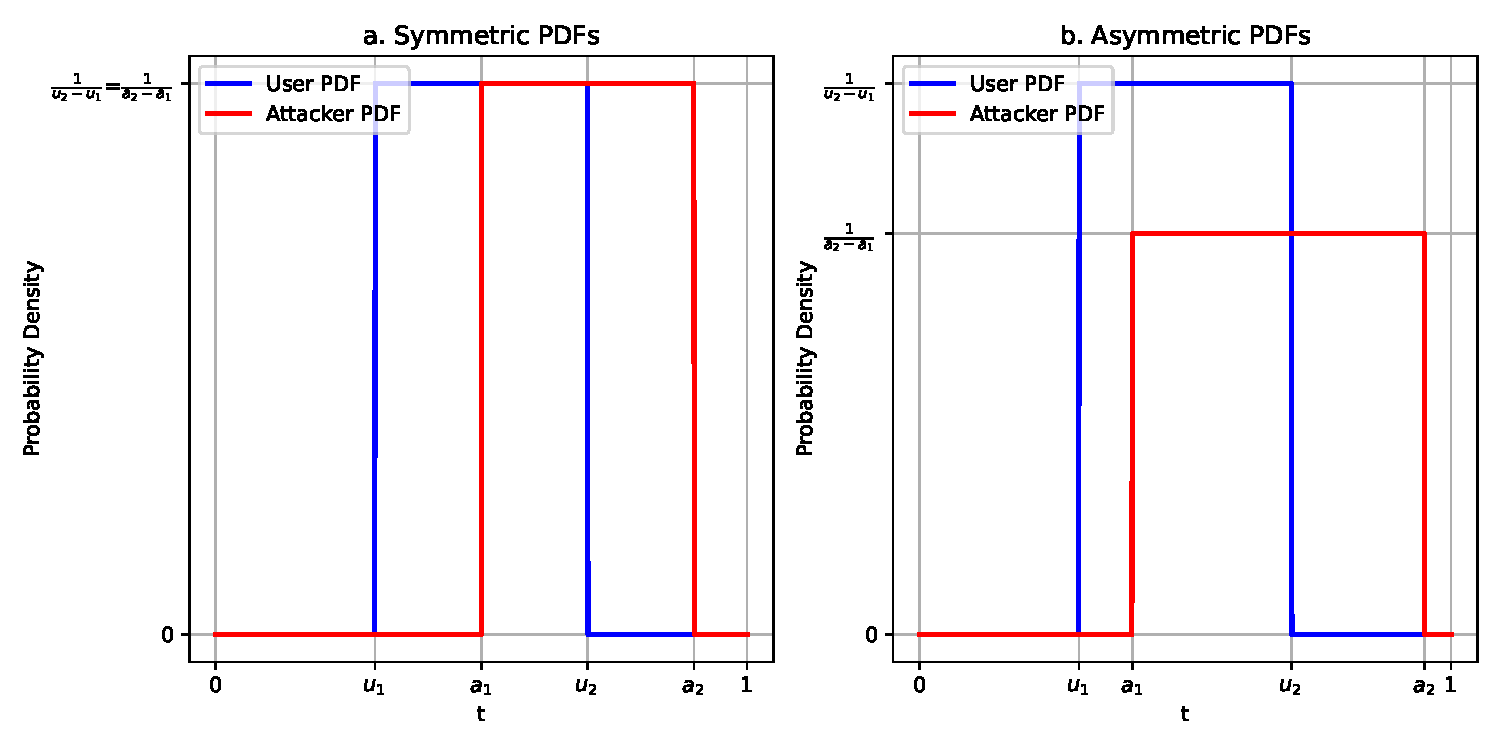
\includegraphics[width=0.995\textwidth]{fig_uniforms.pdf}
    \caption{Symmetric and Asymmetric Uniform PDFs}
\end{figure}

Without loss of generality, we assume that $u_1 < a_1$ and $u_2 < a_2$. Furthemore, we assume there is an overlaping region between the distributions; otherwise the scenario reduces to a trivial case. We also assume that the user and attacker PDFs are do not fully contain one another, as such cases would render them non-separable. Figure 1a illustrates the case where the user and attacker PDF's are symmetric, while Figure 1b illustrates asymmetric PDFs.
The probability of success for a single credential wallet is defined as:
\[
P_{\text{success}}(w^{\text{single}}) = P_{{\text{safe}}} = 1-\mathrm{P_{\text{loss}}}-\mathrm{P_{\text{leak}}}-\mathrm{P_{\text{theft}}}=1-\mathrm{FRR} - \mathrm{FAR} + \mathrm{FRR} \cdot \mathrm{FAR}
\]

Let $T$ denote the threshold. Then the False Acceptance Rate (FAR) and False Rejection Rate (FRR) are defined as:
\[
\text{FAR}(T) = \int_{a_1}^{T} \frac{1}{a_2-a_1} dt =
\left\{
\begin{array}{ll}
0 & \text{if } T \le a_1 \\
\frac{T-a_2}{a_2 - a_1} & \text{if } a_1 < T \le a_2 \\
1 & \text{if } T > a_2
\end{array}
\right.
\]

\[
\text{FRR}(T) = \int_{T}^{u_2} \frac{1}{u_2-u_1} dt =
\left\{
\begin{array}{ll}
1 & \text{if } T \le u_1 \\
\frac{u_2-T}{u_2 - u_1} & \text{if } u_1 < T \le u_2 \\
0 & \text{if } T > u_2
\end{array}
\right.
\]

We defined the probability of success as a function of the threshold $T$ by setting the $FAR(T)$ $FRR(T)$ into the equation and received:
\[
P_{\text{success}}(T) = 
\left\{
\begin{array}{ll}
    0 & \text{if } T \le u_1 \\
    1 - \frac{u_2-T}{u_2-u_1} & \text{if } u_1 < T \le u_1 \\
    1 - \frac{T-a_1}{a_2-a_1} - \frac{u_2-T}{u_2-u_1} + \frac{(T-a_1)(u_2-T)}{(a_2-a_1)(u_2-u_1)} & \text{if } a_1 < T \le u_2 \\
    1 - \frac{T-a_1}{a_2-a_1} & \text{if } u_2 < T \le a_2 \\
    0 & \text{if } T > a_2
    \end{array}
\right.
\]

$P_{\text{success}}(T)$ is a continuous function in $[u_1,a_2]$ ,differentiable in $(u_1,a_2)$ and maintains 

$P_{\text{success}}(u_1) = P_{\text{success}}(a_2)$ thus by Rolle's Theorem, there exists at least one point in $(u_1,a_2)$ such that:
\[\frac{d}{dT} P_{\text{success}}(T) = 0.\] 

The horizontal tangent point is:

\[
T = \frac{a_2+u_1}{2} \quad \text{for } a_1 \leq T \leq u_2
\]

\[\frac{d}{dt} P_{\text{success}}(T) > 0 \text{, For every } T \in (u_1, \frac{a_2+u_1}{2}) \]

\[\frac{d}{dt} P_{\text{success}}(T) < 0 \text{, For every } T \in (\frac{a_2+u_1}{2}, a_2) \]

Thus, by the First Derivative Test the maximum point is at $T = \frac{a_2+u_1}{2}$.
\[
P_{\text{success}}(T_{\text{opt}}) = \frac{(a_2 - u_1)^2}{4(u_2 - u_1) \cdot(a_2 - a_1)} 
\]
We calculated the EER point and showed it is not equal to the optimal point:
\[
T_{\text{EER}} = \frac{a_1 \cdot u_1 - a_2 \cdot u_2}{u_2 - u_1 + a_2 - a_1} \neq \frac{a_2 + u_1}{2}
\] 
The maximum point represnents the optimal threshold of the wallet. By selecting the threshold value, we influnce the wallet's security sensetivity by adjusting the probability associated with each state in $S$. The optimal point indicates that increasing the offset between the two uniform distributions is likely to improve the wallet's success. This optimal point suggest an asymmetry between the user’s and the attacker’s distribution intervals.. Figure 2 illustrates the probability of success for a single credential wallet depends on the threshold $T$. Figure 3 illustrated the FAR vs FRR curve.

\begin{figure}[H]
    \centering
    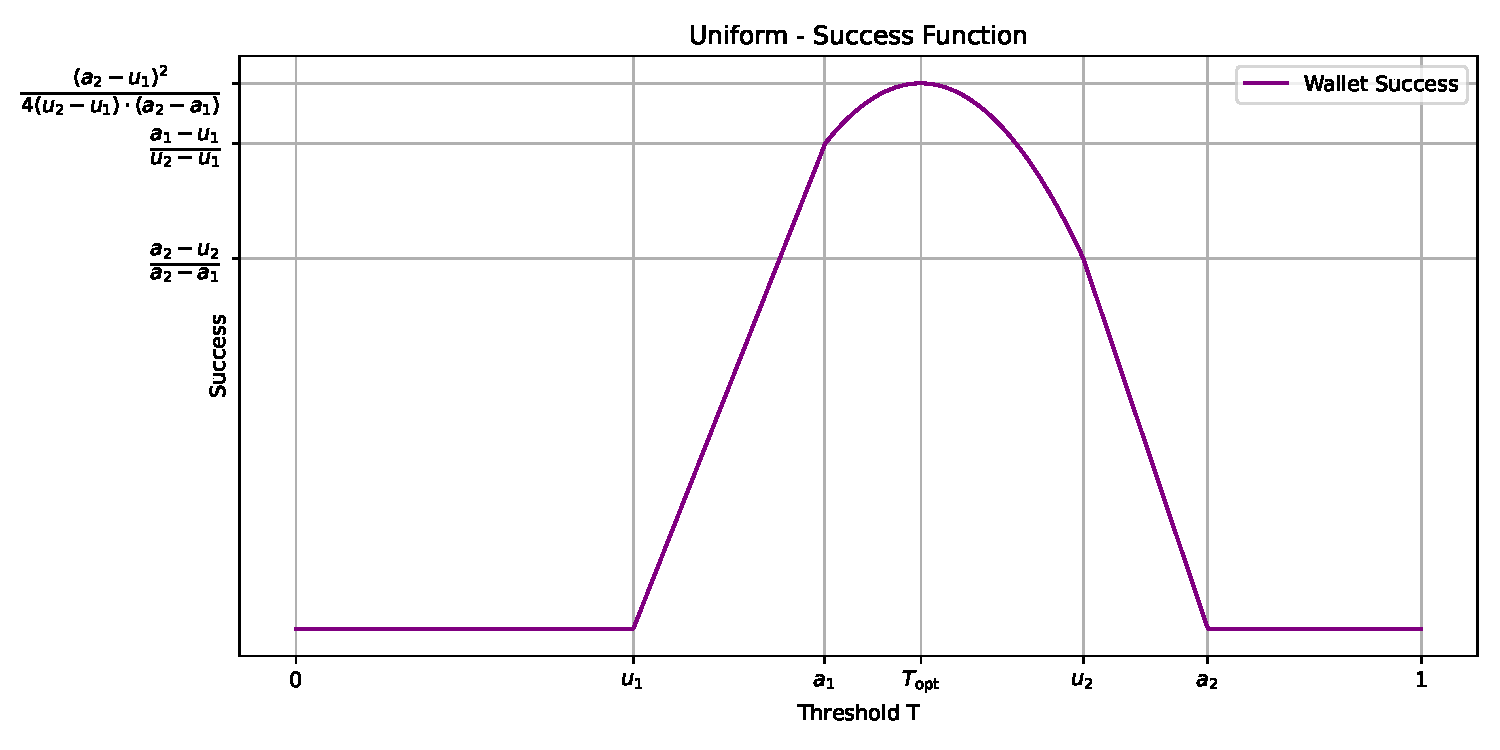
\includegraphics[width=0.85\textwidth]{fig_success_uniform.pdf}
    \caption{Probability of success for a single credential wallet asymmetric uniformly distributed}
\end{figure}
\begin{figure}[H]
    \centering
    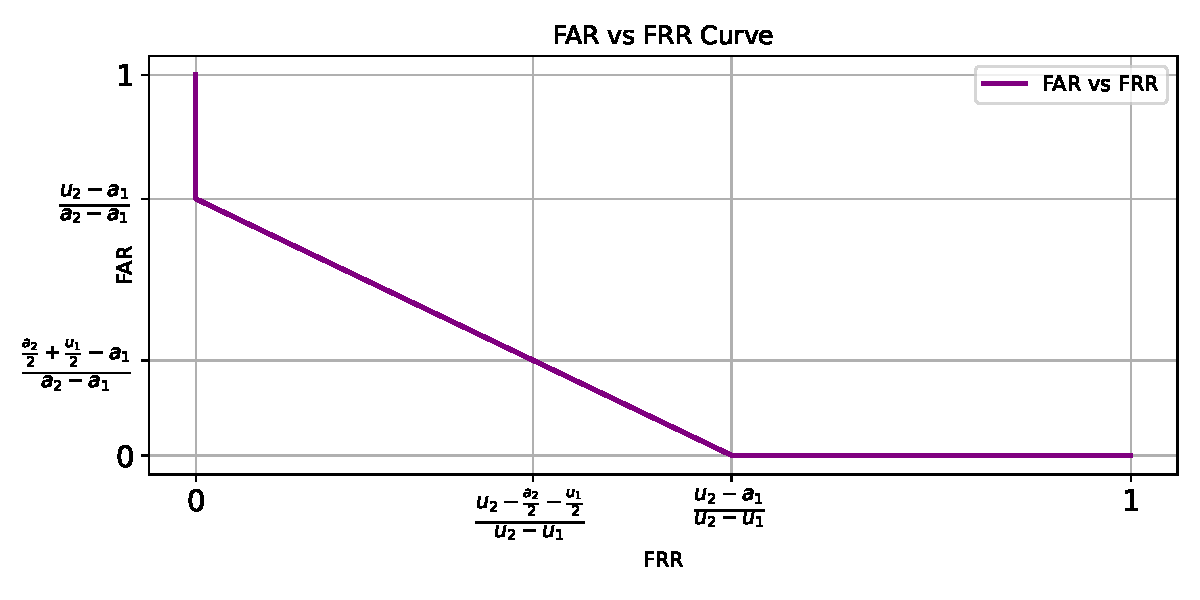
\includegraphics[width=0.75\textwidth]{fig_FARvFRR_uniform.pdf}
    \caption{FAR vs FRR curve}
\end{figure}

\subsubsection{Parabolic Distributed Credential}
%%%
%%%
%%%

\subsection{2 Credentials}
$\{c_1, c_2, \ldots, c_n\}$
\[
P_{\text{Success\_AND}} = \mathrm{P_{\text{safe1}}} \cdot \mathrm{P_{\text{safe2}}} + \mathrm{P_{\text{safe1}}} \cdot \mathrm{P_{\text{leak2}}} + \mathrm{P_{\text{safe2}}} \cdot \mathrm{P_{\text{leak1}}}
\]

\[
P_{\text{Success\_OR}} = \mathrm{P_{\text{safe1}}} \cdot \mathrm{P_{\text{safe2}}} + \mathrm{P_{\text{safe1}}} \cdot \mathrm{P_{\text{loss2}}} + \mathrm{P_{\text{safe2}}} \cdot \mathrm{P_{\text{loss1}}}
\]
\subsection{Symmetric Uniform Distribution Function}
\subsection{Symmetric Parabolic Distribution Function}
%%%
%%%
%%%
\section{Asymmetric Distribution Function}
\subsection{Asymmetric Gaussian Distribution Function}
\subsection{Asymmetric Uniform Distribution Function}
\subsection{Asymmetric Parabolic Distribution Function}
%%%
%%%
%%%
\section{Model}
\subsection{Mechanism Success 2 credentials}
\subsection{Mechanism Success 3 credentials}
%%%
%%%
%%%
\section{Optimal Mechanism}
%%%
%%%
%%%
\section{Conclusion}
%%%
%%%
%%%
\begin{thebibliography}{9}

\bibitem{hong1998}
Lin Hong and Anil Jain.
\textit{Integrating Faces and Fingerprints for Personal Identification}.\\
IEEE Transactions on Pattern Analysis and Machine Intelligence, 1998.

\bibitem{prabhakar2003}
S. Prabhakar, S. Pankanti, and A. K. Jain.\\
\textit{Biometric recognition: Security and privacy concerns}.\\
IEEE Security \& Privacy, 1(2), 33–42, 2003.

\bibitem{sarkar2020}
Arpita Sarkar and Binod K. Singh.\\
\textit{A review on performance, security and various biometric template protection schemes for biometric authentication systems}.\\
Multimedia Tools and Applications, vol. 79, nos. 37–38, pp. 27721–27776, Oct. 2020.

\bibitem{mouallem2024}
Marwa Mouallem and Ittay Eyal.\\
\textit{Asynchronous Authentication}.\\
CCS 2024 - Proceedings of the 2024 ACM SIGSAC Conference on Computer and Communications Security, pp. 3257–3271.

\bibitem{Eyal2021}
Ittay Eyal.\\
\textit{On cryptocurrency wallet design.}.\\
Cryptology ePrint Archive, Paper 2021/1522,2021. https://eprint.iacr.org/2021/1522.
\end{thebibliography}

\end{document}
